\documentclass[10pt]{article}
\usepackage{NotesTeX}
\usepackage{lipsum}
\usepackage{tensor}
\usepackage{amsmath,amsthm,amssymb}
\usepackage{hyperref}
\usepackage{indentfirst}
\usepackage{mathrsfs}

\newcommand{\bs}{\textbackslash}


\title{{\Huge General Relativity}\\{\Large{Class 36 --- April 22, 2020}}} %replace with class number
\author{Chris Layden}

\emailAdd{cplayden777@utexas.edu} %replace with your email
\begin{document}
    \maketitle
    \flushbottom
    \newpage
    \pagestyle{fancynotes}
    \part{The Weak Field Approximation}
	
\section{The Solution to the Wave Equation}
As previously discussed, when working in the weak field approximation, we define our metric to be the flat space metric with a slight perturbation:
              	
\begin{align}\label{eq:weak_metric}
g_{\mu\nu} = \eta_{\mu\nu} + h_{\mu\nu} \hspace{2 cm} |h_{\mu\nu}| << 1 \;.
\end{align}
              	
We eventually noticed that it was much simpler to solve Einstein's equations to find equations of motion using the trace-reversed metric perturbation,
              	
\begin{align}\label{eq:trace_reversed}
\overline{h}_{\mu\nu} = h_{\mu\nu} - \frac{1}{2} h\;,
\end{align}
              	
\noindent where $h = \tensor{h}{^\mu_\mu}$ is the trace of the metric perturbation. Also, recall that we have the ability to perturb our coordinates by a small amount, inducing a gauge transformation on the perturbed metric. If we in particular choose the Lorenz gauge, in which $\partial_\mu \tensor{\overline{h}}{^\;^\mu^\nu} = 0$, Einstein's equations of motion become simply
              	
\begin{align}\label{eq:wave_eqn}
\Box \overline{h}_{\mu\nu} = 16 \pi T_{\mu\nu}\;.
\end{align}
              	
This equation has a formal solution, given by
              	
\begin{align}\label{eq:FormalSln}
\overline{h}^{\mu\nu}(t,x^i) =  4\int d^3 x' \; \frac{T^{\mu\nu}(t_r,(x')^i)}{|x^i-(x')^i|} \;.
\end{align}
              	
              	              	
\begin{figure}[h]
\centering
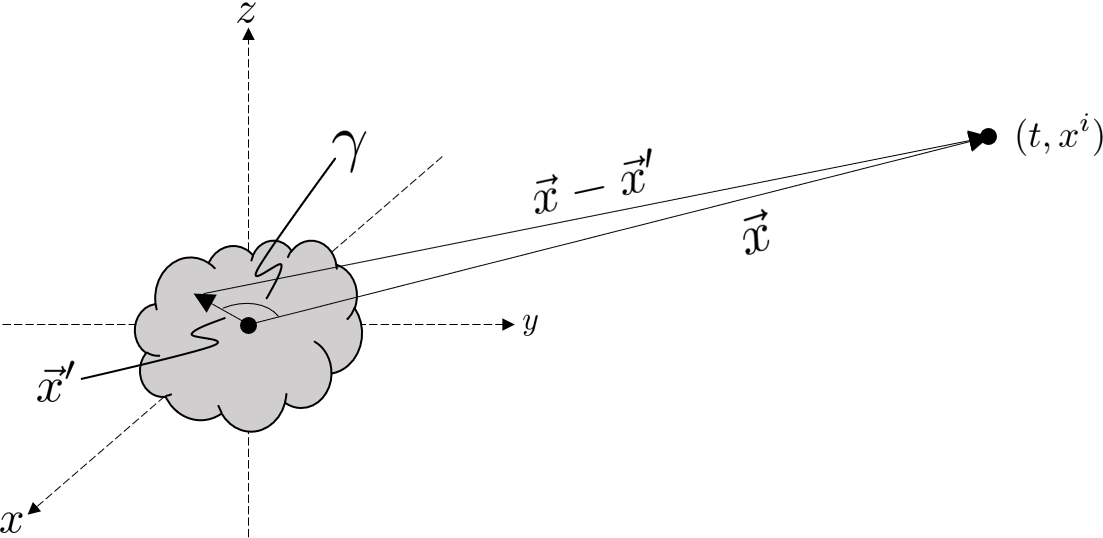
\includegraphics[height=5cm]{FormalSln.png}
\caption{A point $(t,x^i$) in relation to a source of mass/energy.}
\label{fig:FormalSln}
\end{figure}
              	
To help understand what's going on in this equation, consider Fig. \ref{fig:FormalSln}. If we seek to determine the trace-reversed metric $\overline{h}^{\mu\nu}$ at some point $(t,x^i)$ far away from a source of mass/energy, we must integrate over the volume of the source. We do this by labelling any point within the source with a vector $\vec{x'}$ and integrating over $d^3x'$. Over this volume, we integrate the stress-energy tensor $\tensor{T}{^\mu^\nu}$ divided by the distance between $\vec{x'}$ and $\vec{x}$, $|x^i-(x')^i|$. In perhaps more familiar notation,
              	
\begin{align}\label{eq:distanceMag}
|x^i-(x')^i| = \sqrt{(x^i-(x')^i)(x^j-(x')^j) \; \delta_{ij}}\;.
\end{align}
              	
              	
However, we must also be careful that we do not take the value of $\tensor{T}{^\mu^\nu}((x')^i)$ at the same time $t$ for which we desire $\overline{h}^{\mu\nu}(t,x^i)$, because it takes time for any piece of the source at point $\vec{x'}$ to exert an influence on the point $\vec{x}$. Instead, we take $\tensor{T}{^\mu^\nu}$ at a time $t_r$ which is smaller than $t$, such that the influence of a source at $\vec{x'}$ at time $t_r$ arrives at $\vec{x}$ right at time $t$. Since this influence travels at the speed of light, we can define $t_r$, called the \textit{retarded time}, as:
              	
\begin{align}\label{eq:retardedTime}
t_r = t - |x^i-(x')^i| \;.
\end{align}
              	
To understand the relationship between the sources and the trace-reversed metric at a point $(t,x^i)$, consider Fig. \ref{fig:timeInfluence}. In this figure, which suppresses one spatial dimension, a  past-directed light cone emanates from $(t,x^i)$. A cylinder represents the boundary of all of the sources in the spacetime. Since the influence of these sources propagates at the speed of light, the only points at which these sources may influence $\overline{h}^{\mu\nu}(t,x^i)$ (and thus, the only points we want to integrate over) are those points which intersect the light cone, shaded in grey. This is why we integrate $\tensor{T}{^\mu^\nu}$ at $t_r$ rather than at $t$; the points in the shaded region have some value for $t_r < t$ determined by their distance from $(t,x^i)$.
              
\begin{figure}[h]
\centering
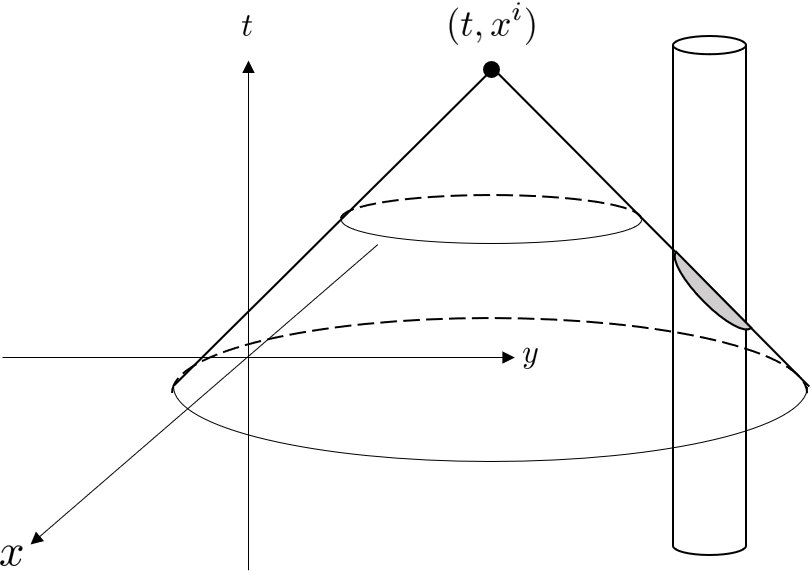
\includegraphics[height=5cm]{timeInfluence.png}
\caption{For a source localized in the cylinder, the only points which influence the trace-reversed metric at $(t,x^i)$ are those in the shaded region.}
\label{fig:timeInfluence}
\end{figure}
                
Eq. \ref{eq:FormalSln} is completely analogous to the solution of the wave equation in electromagnetism - even the concept of retarded time. For a complete derivation of Eq. \ref{eq:FormalSln} from the wave equation, Eq. \ref{eq:wave_eqn}, see Jackson's Classical Electrodynamics.
                
\begin{figure}[h]
\centering
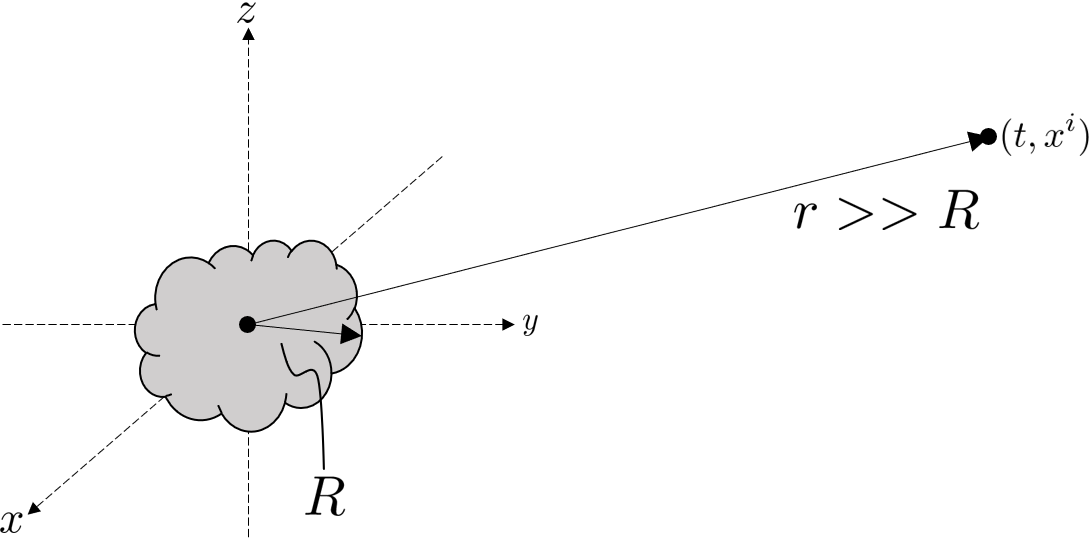
\includegraphics[height=5cm]{distantSource.png}
\caption{Considering a point far from the source.}
\label{fig:distantSource}
\end{figure}
                
Now, we often consider cases for which $x^i$ is far away from any sources, as demonstrated in Fig. \ref{fig:distantSource}. Therefore, if we denote $r = \sqrt{x^ix_i}$ to be the distance to the point $x^i$ at which we seek the metric, $r' = \sqrt{(x')^i(x')_i}$ to be the distance to any point in the source, and $R = max(r')$ to be the distance to the "farthest out" point in the source, then we may assume that $r >> R$.
                
This assumption allows us to simplify the quantity $\frac{1}{|x^i-(x')^i|}$. Firstly, we notice that
                
\[ \frac{1}{|x^i-(x')^i|} = ((x^i-(x')^i)(x^j-(x')^j) \; \delta_{ij})^{-\frac{1}{2}} \]
                
\[= (r^2 + (r')^2 - 2 x^i (x')_i)^{-\frac{1}{2}} = \frac{1}{r} \left( 1 - \frac{2 x^i (x')_i}{r^2} + \left( \frac{r'}{r}\right)^2 \right) ^{-\frac{1}{2}}\] \; .
                
Since we are assuming that $r >> r'$, the terms in the parentheses look like $(1 + x)$ for some small x. Then, using the binomial approximation, we can simplify the expression to 
                
\[ \frac{1}{r}\left( 1 + \left(-\frac{1}{2}\right) \left( - \frac{2 x^i (x')_i}{r^2} + \left( \frac{r'}{r}\right)^2 \right) \right) =   \frac{1}{r}\left( 1 + \frac{x^i (x')_i}{r^2} - \left( \frac{1}{2} \right) \left( \frac{r'}{r}\right)^2 \right) \; .\]
                
Now, observe that within the parentheses, the second term is of order $\frac{1}{r}$, since the $x^i$ in the numerator is of order $r$; the third term, however, is of order $\frac{1}{r^2}$. Since we assume that $r >> r'$, we can neglect this third term. So we now have
                
\begin{align}\label{eq:sourceSimplify}
\frac{1}{|x^i-(x')^i|} = \frac{1}{r} + \frac{x^i (x')_i}{r^3} + O\left(\frac{1}{r^3}\right) \; .
\end{align}
                
Alternatively, we could express this approximation by thinking of $x^i (x')_i$ as a 3-dimensional dot product, $\vec{x} \cdot \vec{x'}$. Then we may write $x^i (x')_i = \vec{x} \cdot \vec{x'} = r r' \cos{\gamma}$, where $\gamma$ is the angle between $\vec{x}$ and $\vec{x'}$, as shown in Fig. \ref{fig:FormalSln}. Thus Eq. \ref{eq:sourceSimplify} becomes simply
                
\begin{align}\label{eq:sourceSimplifyAngle}
\frac{1}{|x^i-(x')^i|} = \frac{1}{r} + \frac{r'\cos{\gamma}}{r^2} + O\left(\frac{1}{r^3}\right) \; .
\end{align}
                
Eq. \ref{eq:sourceSimplifyAngle} can actually be thought of as just the first term in an expansion for $\frac{1}{|x^i-(x')^i|}$ which is accurate to all orders:
                
\begin{align}\label{eq:legendre}
\frac{1}{|x^i-(x')^i|} = \frac{1}{r} \sum_{l=0}^{\infty} \frac{r'}{r} P_l(\cos{\gamma})
\end{align}
                
\noindent where $P_l$ are the Legendre polynomials.
                
Before we move on, let's note the useful fact that, due to conservation of the stress-energy tensor, $\partial_\mu T^{\mu\nu}=0$ (where we approximate the covariant derivative using the partial derivative in our approximately flat space), and so we have
                
\begin{align}\label{eq:stressConservation}
\partial_0 T^{0\nu} = -\partial_i T^{i\nu} \; .
\end{align}
                
As an example of how Eq. \ref{eq:stressConservation} can come in handy, let's consider the following integral over a spatial hypersurface:
                
\[ \int_\Sigma d^3 x \; \partial_i (x^j T^{i\nu}) \; .\]
                
 Notice that since this is an integral of a total derivative over a spatial hypersurface $\Sigma$, we may apply Stokes' Theorem to convert the integral to a surface integral over the boundary of $\Sigma$, $\partial\Sigma$:
                
\[ \int_\Sigma d^3 x \; \partial_i (x^j T^{i\nu}) = \int_{\partial\Sigma} d^2 x \; (x^j T^{i\nu})s_i \; .\]
                
\noindent Where $s_i$ is the normal vector to the surface $\partial\Sigma$. However, at this infinitely far away boundary, $T^{\mu\nu} = 0$, since we are considering a localized source. So the original integral is zero. We could have also expressed the integral by expanding out via the product rule:
                
\[ 0 = \int d^3 x \; \partial_i (x^j T^{i\nu}) = \int d^3x \;\left( \delta^i_j T^{i\nu} + x^j \partial_i T^{i\nu} \right)\]
                
                
\[ = \int d^3 x \; T^{j\nu} - \int d^3 x \; (x^j \partial_0 T^{0\nu}) \]
                
where we applied Eq. \ref{eq:stressConservation}. And thus we have
                
\begin{align}\label{eq:stressIdentity}
\int d^3 x \; T^{j\nu} = \int d^3 x \; (x^j \partial_0 T^{0\nu}) \; .
\end{align}
                
This type of trick, in which we can replace an integral over something like $T^{j\nu}$ with an integral which includes a time derivative, will be useful especially when considering static sources.
             
\section{Static Sources}
We now turn our attention to cases in which the source does not change with time, such that $T^{\mu\nu}$ is a function of $x^i$ only. Thus, $\partial_0 T^{0\nu} = 0$, and by Eq. \ref{eq:stressConservation}, $\partial_i T^{i\nu} = 0$ as well. Also, by Eq. \ref{eq:stressIdentity}, 

\begin{align}\label{eq:Tidentity}
\int d^3 x' \; T^{j\nu} = 0 \; .
\end{align}

Now, let's look at the component $\overline{h}^{00}$ of the trace-reversed metric perturbation. From our formula presented in Eq. \ref{eq:FormalSln} and plugging in our simplification for $\frac{1}{|x^i-(x')^i|}$ given in Eq. \ref{eq:sourceSimplify}, we see that

\[ \overline{h}^{00} = 4 \int d^3x' \; \frac{T^{00}}{r} \left( 1 + \left( \frac{x^j(x')_j}{r^3} \right) \right) + O\left(\frac{1}{r^3}\right)\]

\begin{align}\label{eq:h00long}
= \frac{4}{r} \int d^3x' \; T^{00} + \frac{4 x_j}{r^3} \int d^3x' \; (x')^j T^{00} +  O\left(\frac{1}{r^3}\right) \; .
\end{align}
                
Now, recall that $T^{00}$ in flat space is simply the density. Therefore, the first integral - this density integrated over all space - should yield the total mass of the source, $M$. This first term is the 0th moment of the mass distribution, because it involves no powers of $x$. 

The second term is called the first moment of the mass distribution, as it is dependent on one power of $x$. The terms of order $ O\left( \frac{1}{r^3} \right)$, which we often neglect, would give us even more moments of the distribution. Notice that, in the second term (the first moment), we integrate the product of position and the density of the source at that position - a similar prescription as for determining the center of mass of the source. In fact, if divided by the total mass $M$ of the source, this integral would yield the center of mass. The integral $\int d^3x' \; (x')^j T^{00}$ is called the \textit{mass dipole moment}, and it is frequently denoted $D^j$. 

Now, note that we may always choose our coordinates such that the origin is set at the center of mass of our source. Following this practice, $D^j = 0$, and 

\begin{align}\label{eq:h00}
\overline{h}^{00} =\frac{4}{r} \int d^3x' \; T^{00} +  O\left(\frac{1}{r^3}\right) \approx \frac{4M}{r}\; .
\end{align}

Let's march on and calculate the other components of $\overline{h}^{\mu\nu}$, starting with $\overline{h}^{0j}$:

\[ \overline{h}^{0j} = \frac{4}{r} \int d^3x' \; T^{0j} \left( 1 + \left( \frac{x_k(x')^k}{r^2} \right) \right) + O\left(\frac{1}{r^3}\right) \; . \]

\noindent We then note that the first term in this integral will be zero, by Eq. \ref{eq:Tidentity}. So we are left with

\[ \overline{h}^{0j} = \frac{4x_k}{r^3} \int d^3x' T^{0j} (x')^k + O\left(\frac{1}{r^3}\right)\; . \]

In Homework 8, you will show that the integral above has the property

\begin{align}\label{HWidentity}
\int d^3x' T^{0j} (x')^k = - \int d^3x' T^{0k} (x')^j \;
\end{align}

\noindent and, using this identity, you will also show that $\overline{h}^{0j}$ may be expressed as

\begin{align}\label{eq:h0j}
\overline{h}^{0j} = \frac{2\tensor{\epsilon}{^j_k_m} J^k x^m}{r^3}
\end{align}

\noindent where

\begin{align}\label{eq:currentDipole}
J^k = \int \tensor{\epsilon}{^k_a_b} (x')^a T^{0b} d^3 x' \; .
\end{align}

Note that, in traditional 3D calculus, the contraction of two indices of the Levi-Civita tensor into two vectors has the interpretation of the cross product between the vectors. In the case of Eq. \ref{eq:currentDipole}, one of these vectors, $T^{0b}$, is momentum density, which we might denote as the vector $\mathscr{P}^b$. Therefore, we can interpret $\tensor{\epsilon}{^k_a_b} (x')^a T^{0b} = \vec{x'} \times \vec{\mathscr{P}}$ as an angular momentum density. Since $J^k$ is this angular momentum density integrated over all of space, $J^k$ has the interpretation of the total angular momentum of the source. $J^k$ is also known as the \textit{current dipole moment} of the mass distribution, since it depends on the motion of the sources and contains one power of $x$.

Lastly, we can compute $\overline{h}^{ij}$:

\[ \overline{h}^{ij} = \frac{4}{r} \int d^3x' \; T^{ij} \left( 1 + \left( \frac{x_k(x')^k}{r^2} \right) \right) + O\left(\frac{1}{r^3}\right) \; . \]

Once again, the first term of the integral is 0 by application of Eq. \ref{eq:Tidentity}. So

\[ \overline{h}^{ij} = \frac{4x_k}{r^3} \int d^3x' \; T^{ij} (x')^k + O\left(\frac{1}{r^3}\right) \; . \]

However, Eq. \ref{HWidentity} may in fact be extended to show that 

\[ \int d^3x' \; T^{\mu j} (x')^k = - \int d^3x' \; T^{\mu k} (x')^j \; . \]

Thus, using in addition the symmetry of $T^{\mu\nu}$,

\[ \int d^3x' \; T^{ij} (x')^k =  \frac{1}{2} \int d^3x' \; \left( T^{ij}(x')^k + T^{ji} (x')^k \right) = -\frac{1}{2} \int d^3x' \; \left( T^{ik}(x')^j + T^{jk} (x')^i \right)\]

\[ = - \frac{1}{2} \int d^3x' \; \left( T^{ki}(x')^j + T^{jk} (x')^i \right) = - \frac{1}{2} \int d^3x' \; \left( - T^{kj}(x')^i + T^{jk} (x')^i \right) = 0 \; .\]

So we find $\overline{h}^{ij} = O\left(\frac{1}{r^3}\right) \approx 0$. We now have all of the components of $\overline{h}^{\mu\nu}$. But we would like to find the metric itself, so we need the components of $h^{\mu\nu}$. We may find the trace of $\overline{h}^{\mu\nu}$, $\overline{h} = \tensor{\overline{h}}{^\mu_\mu}$ as follows:

\begin{align}\label{htrace}
\overline{h} = \overline{h}^{\mu\nu} \eta_{\mu\nu} = -\overline{h}^{00} + \sum_j \overline{h}^{jj} = -\frac{4M}{r} + O\left(\frac{1}{r^3}\right) \; .
\end{align}

And so, trace-reversing $\overline{h}^{\mu\nu}$ to get back to $h^{\mu\nu}$:

\[ h^{\mu\nu} = \overline{h}^{\mu\nu} - \frac{1}{2} \overline{h} \;  \eta^{\mu\nu} \]

\[ \rightarrow h^{00} = \overline{h}^{00} + \frac{1}{2} \overline{h} = \frac{4M}{r} + \frac{1}{2}\left( - \frac{4M}{r}\right) = \frac{2M}{r}\]

\[ \rightarrow h^{0j} = \overline{h}^{0j} = \frac{2\tensor{\epsilon}{^j_k_m} J^k x^m}{r^3}\]

\[ \rightarrow h^{ij} = - \frac{1}{2}\left( - \frac{4M}{r}\right) = \frac{2M}{r} \; .\]

Now, converting to $h_{\mu\nu} = h^{\alpha\beta} \eta_{\alpha\mu} \eta_{\beta\nu}$:

\[ h_{00} = \frac{2M}{r}(-1)(-1) = \frac{2M}{r}\]
\[ h_{ij} = h^{ij}(1)(1) = h^{ij} \]
\[ h_{0i} = h^{0i}(-1)(1) = -h^{0i} \; .\]

Finally, we can calculate the metric $g_{\mu\nu}$ itself via Eq. \ref{eq:weak_metric}. We may then write the line element as follows:

\begin{align}\label{lineElement}
ds^2 = g_{\mu\nu} dx^\mu dx^\nu = -\left( 1-\frac{2M}{r} \right) dt^2 - \frac{2\tensor{\epsilon}{^j_k_m} J^k x^m}{r^3}(dtdx^j + dx^j dt) + \left( 1 + \frac{2M}{r} \right) \delta_{ij} dx^i dx^j \; .
\end{align}

To write this metric in another way, let's assume we orient our axes such that $\vec{J}$ points along the z axis: $\vec{J} = J\hat{z}$. Let's then use spherical polar coordinates. We uncover:

\begin{align}\label{eq:lineElementSpherical}
ds^2 = -\left( 1-\frac{2M}{r} \right) dt^2 - \frac{2J \sin^2{\theta}}{r}(dt d\phi + d\phi dt) + \left( 1 + \frac{2M}{r} \right)(dr^2 + r^2 d\Omega^2) \; .
\end{align}

\section{Motion in the Weak Field Limit}
While we previously required our sources (and thus the metric) to be static, we will now consider metrics which may be dynamic, so long as they satisfy Eq. \ref{eq:weak_metric}. We can investigate motion in the weak field limit by considering the geodesic equation. For the paths of massive particles, we are going to use the affine parameter $\lambda = \frac{\tau}{m}$, while for massless particles we will use the same affine parameter $\lambda$ we have been using. This allows us to write $\frac{dx^\mu}{d\lambda}=p^\mu$ and

\begin{align}\label{eq:momentumRelation}
p^t = \frac{dt}{d\lambda} = E
\end{align}

\noindent for both massive and massless particles, as for massive particles $\frac{dt}{d\lambda}= m\frac{dt}{d\tau} = m\gamma = E$. For massive particles, we may also write that $p^i = \frac{dx^i}{d\lambda} = m\frac{dx^i}{d\tau} = m\gamma v^i = Ev^i$. Recall that the geodesic equation takes form

\begin{align}\label{eq:geodesicEq}
\frac{dp^\mu}{d\lambda} + \Gamma^\mu_{\alpha\beta} p^\alpha p^\beta = 0 \; .
\end{align}

\noindent Note that we could write the first term $\frac{dp^\mu}{d\lambda}$ as $\frac{dp^\mu}{dt}\frac{dt}{d\lambda} = E \frac{dp^\mu}{dt}$. We can see that Eq. \ref{eq:geodesicEq} has terms only up to order $v^2$. We will often neglect the terms of order $v^2$, but they could be written out if desired. Let's first consider the $\mu = 0$ term in Eq. \ref{eq:geodesicEq}. In doing so, recall that $h_{00}$ is related to the Newtonian potential: $h_{00} = -2\Phi$. So we will replace $h_{00}$ with $-2\Phi$ when it arises. We  will also denote $h_{0j} = w_j$. If we compute all of the Christoffel symbols and plug them into Eq. \ref{eq:geodesicEq}, we find that
\begin{align}\label{eq:dp0}
\frac{dp^0}{dt} = \frac{dE}{dt} = -E(\partial_0 \Phi + 2(\partial_k \Phi)v^k) + O(v^2) \; .
\end{align}

From this result, we observe that the change in a particle's energy over time, $\frac{dE}{dt}$, may be caused by changes in the potential $\Phi$ over time or by motion of the particle across a gradient in $\Phi$.

Next, for $\mu = i$ (with the index lowered for convenience), we have

\begin{align}\label{eq:dpi}
\frac{dp_i}{dt} = -E(\partial_i \Phi + \partial_0 w_i + 2 \partial_{[i} w_{j]} v^j + 2 \partial_0 h_{ij} v^j) + O(v^2) \; .
\end{align}

Let's break this expression down piece by piece. The first term in the parentheses, $\partial_i \Phi$, is just a gradient of the potential, so it seems to have the usual interpretation of a force. But additionally, the first and second terms combined look like how we might build the electric field via an electric potential and vector potential. With this intuition, let's construct the object

\begin{align}\label{eq:Gi}
G_i = \partial_i \Phi + \partial_0 h_{0i} = \partial_i \Phi + \partial_0 w_i
\end{align}

The electric field $E_i$ obeys an identical expression with the electric potential $\Phi$ and the vector potential $A_i$, since $E_i = \partial_i \Phi + \partial_0 A_i$. Doing some manipulation involving some identities of the Levi-Civita tensor, we can also show the second term in Eq. \ref{eq:dpi}, may be written

\begin{align}\label{eq:gravitomagnetic}
\partial_{[i} w_{j]} v^j = \epsilon_{ikm} v^k H^m \hspace{1 cm} \textrm{where} \hspace{1 cm} H^m = \epsilon^{mab} \partial_a h_{0b} = \epsilon^{mab} \partial_a w_b \; .
\end{align}

Which is just the velocity $\vec{v}$ crossed into this new vector $\vec{H}$. Furthermore, $\vec{H}$ looks like the cross product of the gradient operator with $\vec{w}$ - a curl! So, written in 3D vector notation, the term $\partial_{[i} w_{j]} v^j$ becomes $\vec{v} \times \vec{H}$ for $\vec{H} = \vec{\nabla} \times \vec{w}$. Once again, this looks just like something we've seen in electromagnetism - the magnetic force, where $\vec{H}$ is analogous to the magnetic field $\vec{B} = \vec{\nabla} \times \vec{A}$. So, putting these conclusions together, we can rewrite Eq. \ref{eq:dpi} as

\begin{align}\label{eq:gravitoElectric}
\frac{d\vec{p}}{dt} = -E(\vec{G} + \vec{v} \times \vec{H} + ...)
\end{align}

Note that the remaining terms are not vanishing; they just don't fit into the electromagnetic analogy. But we can interpret the first term in Eq. \ref{eq:gravitoElectric} as a "gravito-electric" force and the second term as a "gravito-magnetic" force, in analogy to the Lorentz force equation $\vec{F} = \frac{d\vec{p}}{dt} = q \vec{E} + q \vec{v} \times \vec{B}$.

Now, let's consider what this "gravito-magnetic" force looks like in the case of static sources. Recall that since $w_j = h_{0j} = -\frac{2 \epsilon_{jkm} J^k x^m}{r^3}$, we may write

\begin{align}\label{eq:wvector}
\vec{w} = \frac{-2\vec{J} \times \hat{n}}{r^2}
\end{align}

\noindent in analogy to the vector potential of a magnetic dipole,

\begin{align}\label{eq:magDipolePotential}
\vec{A} = \frac{\vec{m} \times \hat{n}}{r^2} \;
\end{align}

\noindent if we associate the vector $-2\vec{J}$ with the magnetic dipole moment $\vec{m}$. Then, just as how we would write the magnetic field $\vec{B}= \vec{\nabla} \times \vec{A} $ of a magnetic dipole with moment $-2\vec{J}$, we may expand out $\vec{H} = \vec{\nabla} \times \vec{w}$ using Eq. \ref{eq:wvector} into

\begin{align}\label{eq:gravitoMagMomentum}
\vec{H} = \frac{3(-2\vec{J} \cdot \hat{n}) \hat{n} - (\vec{-2J})}{r^3} \; .
\end{align}

Thus, we can consider a spacetime with angular momentum as having a gravito-magnetic effect which is a dipole at leading order. This effect is suppressed in everyday life by factors of $c$ which are hidden in Eq. \ref{eq:gravitoMagMomentum}. But in the same way that a spinning particle in a magnetic field will precess, as shown in Fig. \ref{fig:GravMag}, a gyroscopic placed in orbit around a spinning body will also precess.

\begin{figure}[h]
\centering
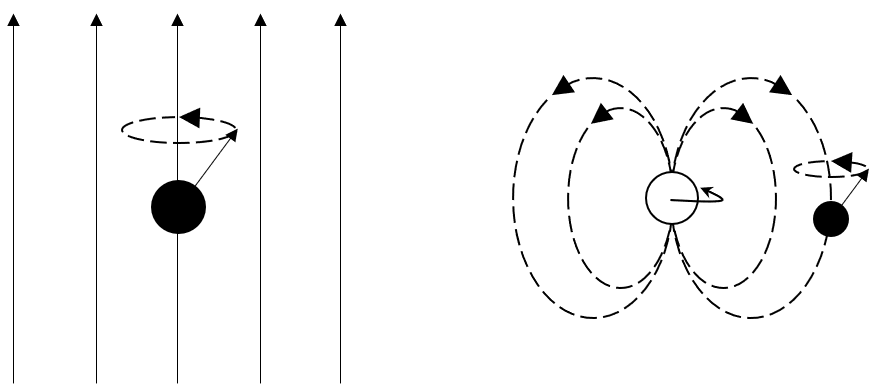
\includegraphics[height=5cm]{gravmag.png}
\caption{A spinning particle in a magnetic field (left) and a gyroscope in orbit about a rotating body (right).}
\label{fig:GravMag}
\end{figure}

\end{document}